\documentclass{beamer}

\usetheme{metropolis}
\definecolor{mediumred}{RGB}{180, 10, 5}
\setbeamercolor{frametitle}{bg=mediumred, fg=white}

\usepackage{tkz-graph}
\usepackage{tikz}
\usetikzlibrary{arrows,matrix,decorations.pathreplacing,positioning,chains,fit,shapes,calc} %
\usetikzlibrary{calc,patterns,decorations.pathmorphing,decorations.markings}

\usepackage{siunitx}

\usepackage{custom}

\title{Computing controlled invariant sets for hybrid systems with applications to model-predictive control}
\date{}
\author{Beno\^it Legat${}^*$, Paulo Tabuada${}^\dagger$ and Rapha\"el M. Jungers${}^*$}
\institute{${}^*$ UCLouvain, ${}^\dagger$ UCLA}

\makeatletter
\let\@@magyar@captionfix\relax
\makeatother

\begin{document}
\maketitle

\begin{frame}
  \frametitle{Contents}
  \tableofcontents
\end{frame}

\section{Safe Model Predictive Control}

\begin{frame}
  \frametitle{Motivating application : Model Predictive Control}
  A truck with $M$ trailers linked by mass-spring dampers.

  \begin{block}{Initial state}
    \vspace{-1em}
    \begin{itemize}
      \item Speed of truck and trailers $v_i = \SI{10}{\meter\per\second}$.
      \item Spring elongation $d_i = \SI{0}{\meter}$.
    \end{itemize}
  \end{block}
  \vspace{-1em}
  \begin{block}{Objective}
    Maximize distance covered in \SI{60}{\second}.
  \end{block}
  \vspace{-.5em}
  \begin{block}{Control}
    Acceleration of truck $|u| \leq \SI{4}{\meter\per\second\squared}$.
  \end{block}
  \vspace{-.5em}
  \begin{block}{\alert{Safety} requirements}
    \vspace{-1em}
    \begin{itemize}
      \item Speed of truck and each trailer $v_i \leq \SI{35}{\meter\per\second}$.
      \item Spring elongation $|d_i| \leq \SI{0.5}{\meter}$.
    \end{itemize}
  \end{block}
  \vspace{-1em}
  \begin{center}
    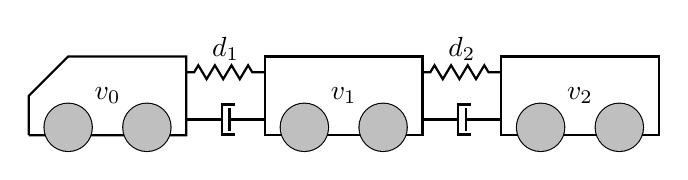
\begin{tikzpicture}
      \tikzstyle{spring}=[thick,decorate,decoration={zigzag,pre length=0.1cm,post length=0.1cm,segment length=6}]
\tikzstyle{damper}=[thick,decoration={markings,
  mark connection node=dmp,
  mark=at position 0.5 with
  {
    \node (dmp) [thick,inner sep=0pt,transform shape,rotate=-90,minimum width=10pt,minimum height=2pt,draw=none] {};
    \draw [thick] ($(dmp.north east)+(2pt,0)$) -- (dmp.south east) -- (dmp.south west) -- ($(dmp.north west)+(2pt,0)$);
    \draw [thick] ($(dmp.north)+(0,-4pt)$) -- ($(dmp.north)+(0,4pt)$);
  }
}, decorate]
\draw[thick] (0, 0) -- (2, 0) -- (2, 1) -- (0.5, 1) -- (0, 0.5) -- (0, 0);
\draw [spring] (2, 0.8) -- (3, 0.8);
\draw [damper] (2, 0.2) -- (3, 0.2);
\draw[thick] (3, 0) rectangle (5, 1);
\draw [spring] (5, 0.8) -- (6, 0.8);
\draw [damper] (5, 0.2) -- (6, 0.2);
\draw[thick] (6, 0) rectangle (8, 1);
\draw[thick] (0.5, 0.1) circle (0.3);
\fill[color=lightgray] (0.5, 0.1) circle (0.3);
\draw[thick] (1.5, 0.1) circle (0.3);
\fill[color=lightgray] (1.5, 0.1) circle (0.3);
\draw[thick] (3.5, 0.1) circle (0.3);
\fill[color=lightgray] (3.5, 0.1) circle (0.3);
\draw[thick] (4.5, 0.1) circle (0.3);
\fill[color=lightgray] (4.5, 0.1) circle (0.3);
\draw[thick] (6.5, 0.1) circle (0.3);
\fill[color=lightgray] (6.5, 0.1) circle (0.3);
\draw[thick] (7.5, 0.1) circle (0.3);
\fill[color=lightgray] (7.5, 0.1) circle (0.3);
\node at (1, 0.5) {$v_0$};
\node at (4, 0.5) {$v_1$};
\node at (7, 0.5) {$v_2$};
\node at (2.5, 1.1) {$d_1$};
\node at (5.5, 1.1) {$d_2$};

    \end{tikzpicture}
  \end{center}
\end{frame}

\begin{frame}{Safety requires \alert{long} horizon}
  Speed limit changes from \SI{35}{\meter\per\second} to \SI{15.6}{\meter\per\second} after \SI{30}{\second}.
  \begin{center}
    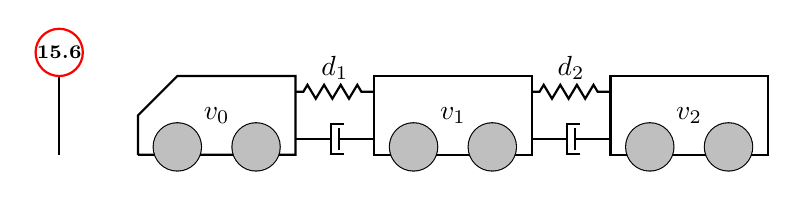
\begin{tikzpicture}
      \tikzstyle{spring}=[thick,decorate,decoration={zigzag,pre length=0.1cm,post length=0.1cm,segment length=6}]
\tikzstyle{damper}=[thick,decoration={markings,
  mark connection node=dmp,
  mark=at position 0.5 with
  {
    \node (dmp) [thick,inner sep=0pt,transform shape,rotate=-90,minimum width=10pt,minimum height=2pt,draw=none] {};
    \draw [thick] ($(dmp.north east)+(2pt,0)$) -- (dmp.south east) -- (dmp.south west) -- ($(dmp.north west)+(2pt,0)$);
    \draw [thick] ($(dmp.north)+(0,-4pt)$) -- ($(dmp.north)+(0,4pt)$);
  }
}, decorate]
\draw[thick] (0, 0) -- (2, 0) -- (2, 1) -- (0.5, 1) -- (0, 0.5) -- (0, 0);
\draw [spring] (2, 0.8) -- (3, 0.8);
\draw [damper] (2, 0.2) -- (3, 0.2);
\draw[thick] (3, 0) rectangle (5, 1);
\draw [spring] (5, 0.8) -- (6, 0.8);
\draw [damper] (5, 0.2) -- (6, 0.2);
\draw[thick] (6, 0) rectangle (8, 1);
\draw[thick] (0.5, 0.1) circle (0.3);
\fill[color=lightgray] (0.5, 0.1) circle (0.3);
\draw[thick] (1.5, 0.1) circle (0.3);
\fill[color=lightgray] (1.5, 0.1) circle (0.3);
\draw[thick] (3.5, 0.1) circle (0.3);
\fill[color=lightgray] (3.5, 0.1) circle (0.3);
\draw[thick] (4.5, 0.1) circle (0.3);
\fill[color=lightgray] (4.5, 0.1) circle (0.3);
\draw[thick] (6.5, 0.1) circle (0.3);
\fill[color=lightgray] (6.5, 0.1) circle (0.3);
\draw[thick] (7.5, 0.1) circle (0.3);
\fill[color=lightgray] (7.5, 0.1) circle (0.3);
\node at (1, 0.5) {$v_0$};
\node at (4, 0.5) {$v_1$};
\node at (7, 0.5) {$v_2$};
\node at (2.5, 1.1) {$d_1$};
\node at (5.5, 1.1) {$d_2$};

      \draw[thick] (-1, 0) to (-1, 1);
      \draw[thick,color=red] (-1, 1.3) circle (0.3);
      \node at (-1, 1.3) {\scriptsize \bf 15.6};
    \end{tikzpicture}
  \end{center}
  One trailer, step-size of \SI{0.4}{\second}, horizon of \SI{9.2}{\second}/23 step-sizes:
  \begin{center}
    \includegraphics[width=0.5\textwidth]{CruiseControlUnsafeSpeed.pdf}~%
    \includegraphics[width=0.5\textwidth]{CruiseControlUnsafeAcceleration.pdf}
  \end{center}
\end{frame}

\begin{frame}{Controlled invariant set}
  \begin{block}{Linear discrete control system}
    \[ x_{k+1} = A x_k + B u_k, \quad x_k \in X, u_k \in U \]
  \end{block}
  \begin{block}{Controlled invariant set}
    Set $S \subseteq X$ \emph{controlled invariant} iff
    \[ \forall x \in S, \exists u \in U \text{ such that } Ax + Bu \in S \]
  \end{block}
  \begin{block}{Safe MPC}
    \begin{itemize}
      \item Compute controlled invariant set $S \subseteq{}$safe set.
      \item Add constraint: state${}\in S$.
    \end{itemize}
  \end{block}
\end{frame}


\begin{frame}{Representation of polyhedral sets}
  \begin{block}{\hrep}
    Representation of polyhedron $S$ as intersection of halfspaces:
    \[ S = \bigcap_{i=1}^m \{\, x \mid a_i^\Tr x \le \beta_i \,\}. \]
    \vspace{-2.5em}
    \begin{itemize}
      \item Computing $A^{-1} S$ is \alert{easy}: $a_i \to A^\Tr a_i$.
      \item Projection is \alert{hard}. Algorithms: Fourier-Motzkin, ...
    \end{itemize}
  \end{block}
  \begin{block}{\vrep}
    Representation of polyhedron $S$ as hull of points/rays:
    \[ S = \convexhull(x_1, \ldots, x_{m_x}) + \conichull(r_1, \ldots, r_{m_r}). \]
    \vspace{-3em}
    \begin{itemize}
      \item Computing $A S$ is \alert{easy}: $x \to A x$, $r \to A r$.
      \item Projection is \alert{easy}: project each point/ray.
    \end{itemize}
  \end{block}
  \vspace{-1em}
  Representation conversion is \alert{hard}. Algorithms: double description,
  quick hull, ...
\end{frame}

\begin{frame}{Unconstrained input without loss of generality}
  \begin{block}{\alert{Constrained} input}
    \[ x_{k+1} = A x_k + B u_k, \quad x_k \in X, \alert{u_k \in U} \]
  \end{block}
  \textbf{\alert{Lift} to \alert{un}constrained input}: $x' = (x, u)$
  \begin{align*}
    x_{k+1} & =
    \begin{pmatrix}
      A & B
    \end{pmatrix}
    x'_k\\
    u_{k+1} & =
    u'_k
  \end{align*}
  where $x'_k \in X' = X \times U$.
\end{frame}


\begin{frame}{Computation of invariant set}
  \vspace{-.5em}
  Linear discrete system : \( x_{k+1} = A x_k \), $x_k \in X$.
  \vspace{-.8em}
  \begin{block}{Pre-image}
    \[ A^{-1}S \triangleq \{\, x \mid Ax \in S \,\} \]
  \end{block}
  \vspace{-.8em}
  \begin{block}{Invariant set}
    Set $S \subseteq X$ \emph{invariant} iff
    \begin{align*}
      \forall x \in S, Ax & \in S &\Leftrightarrow&& AS & \subseteq S &\Leftrightarrow&& S & \subseteq A^{-1}S
    \end{align*}
  \end{block}
  \only<2>{
  \vspace{-.8em}
    \begin{block}{\alert{Polyhedral} computation}
      \begin{align*}
        P_0 & = X\\
        P_{k+1} & = P_k \cap A^{-1} P_k
      \end{align*}
      \vspace{-3em}
      \begin{center}
        \begin{tabular}{ll}
          $A^{-1}$ & easy with \alerthrep\\
          $\cap$   & easy with \alerthrep
        \end{tabular}
      \end{center}
    \end{block}
  }
  \only<3>{
    \begin{block}{\alert{Ellipsoidal} computation}
      \[ C = \{\, x \mid x^\Tr Q x \le 1 \,\} \quad \Rightarrow \quad A^{-1}C = \{\, x \mid x^\Tr A^\Tr Q A x \le 1 \,\} \]
      S-procedure:
      \[ Q - A^\Tr Q A \text{ is PSD}. \]
    \end{block}
  }
\end{frame}

\begin{frame}{Polyhedral computation of controlled invariant set}
  \vspace{-1em}
  \begin{align*}
    P_0 & = X\\
    P_{k+1}
    & = P_k \cap \proj_x \{\, (x, u) \mid Ax + Bu \in P_k \,\}\\
    & = P_k \cap \proj_x [A, B]^{-1} P_k
  \end{align*}
  \vspace{-1em}
  \begin{block}{Not scalable...}
    \begin{center}
      \begin{tabular}{ll}
        $[A, B]^{-1}$ & easy with \alerthrep\\
        $\proj_x$     & easy with \alertvrep\\
        $\cap$        & easy with \alerthrep
      \end{tabular}
    \end{center}
  \end{block}
\end{frame}

\begin{frame}{Unconstrained control to algebraic system}
  \begin{block}{Linear Discrete \alert{Control} System (DT\alert{C}S)}
    \[ x_{k+1} = A x_k + B u_k, \quad x_k \in X \]
  \end{block}
  \begin{block}{Linear Discrete \alert{Algebraic} System (DT\alert{A}S)}
    \[ Ex_{k+1} = A x_k, \quad x_k \in X \]
    Invariant Set $S \subseteq X$ if
    \[ \forall x \in S, \alert{\exists} y \in S : Ey = Ax \]
  \end{block}
  \begin{block}{Reduction}
    The set $S$ is controlled invariant for the DT\alert{C}S iff
    it is invariant for the DT\alert{A}S
    \[ \Pi x_{k+1} = \Pi A x_k, \quad x_k \in X \]
    where $\Pi$ is a projection on $\Image(B)^\perp$.
  \end{block}
\end{frame}


\begin{frame}{Ellipsoidal controlled invariant Set of Algebraic Systems}
  \[ E x_{k+1} = A x_k, \quad x_k \in X \]
  Convex set $S$ invariant iff
  \begin{align*}
    AS & \subseteq ES\\
    (AS)^\circ & \supseteq (ES)^\circ\\
    A^{-\Tr}S^\circ & \supseteq E^{-\Tr}S^\circ
  \end{align*}
  \begin{block}{Ellipsoidal computation}
    \[ C^\circ = \{\, x \mid x^\Tr Q x \le 1 \,\} \quad \Rightarrow \quad A^{-\Tr}C^\circ = \{\, x \mid x^\Tr A Q A^\Tr x \le 1 \,\} \]
    S-procedure:
    \[ E Q E^\Tr - A Q A^\Tr \text{ is PSD}. \]
  \end{block}
\end{frame}



\section{Generalization to Hybrid Systems}

\begin{frame}
  \frametitle{Main obstacle : need to homogenize}
  Safe set in each modes can have different centers
  \footnotesize{(The issue is already present for non-Hybrid System if the safe set is not symmetric)}.

  Homogenization with new variable $z = 1$.
  \begin{center}
    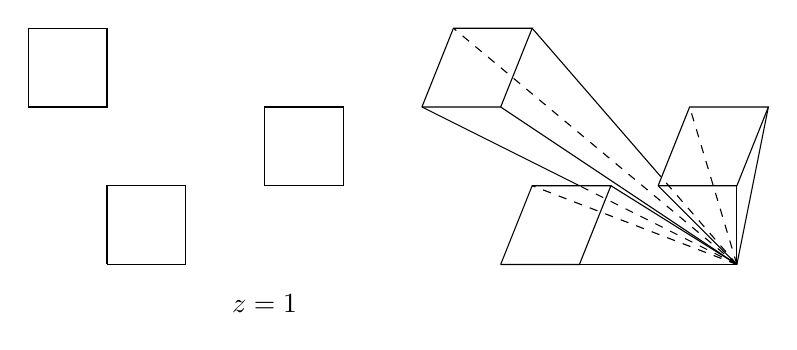
\begin{tikzpicture}
      \draw (0, 0) -- (0, 1) -- (1, 1) -- (1, 0) -- (0, 0);
      \draw (2, 1) -- (2, 2) -- (3, 2) -- (3, 1) -- (2, 1);
      \draw (-1, 2) -- (-1, 3) -- (0, 3) -- (0, 2) -- (-1, 2);

      \node at (2, -0.5) {$z = 1$};
      \draw (5, 0) -- (5.4, 1) -- (6.4, 1) -- (6, 0) -- (5, 0);
      \draw[dashed] (8, 0) -- (5.4, 1);
      \draw (8, 0) -- (6.4, 1);
      \draw (8, 0) -- (6, 0);
      \draw (8, 0) -- (5, 0);
      \draw (7, 1) -- (7.4, 2) -- (8.4, 2) -- (8, 1) -- (7, 1);
      \draw (8, 0) -- (8.4, 2);
      \draw (8, 0) -- (8, 1);
      \draw (8, 0) -- (7, 1);
      \draw[dashed] (8, 0) -- (7.4, 2);
      \draw (4, 2) -- (4.4, 3) -- (5.4, 3) -- (5, 2) -- (4, 2);
      \draw[dashed] (8, 0) -- (6, 1);
      \draw (6, 1) -- (4, 2);
      \draw (8, 0) -- (5, 2);
      \draw[dashed] (8, 0) -- (7, 1.1538);
      \draw (7, 1.1538) -- (5.4, 3);
      \draw[dashed] (8, 0) -- (4.4, 3);
    \end{tikzpicture}
  \end{center}
  We now look for \alert{cones} $K$ instead of \alert{set} $S$.

  We replace \alert{polar} $S^\circ$ with \alert{dual} $K^*$.
\end{frame}

\begin{frame}{Back to our example}
  Four speed limits with a delay $T$ to satisfy limit\\$\to$ \alert{Hybrid} System

  \begin{center}
    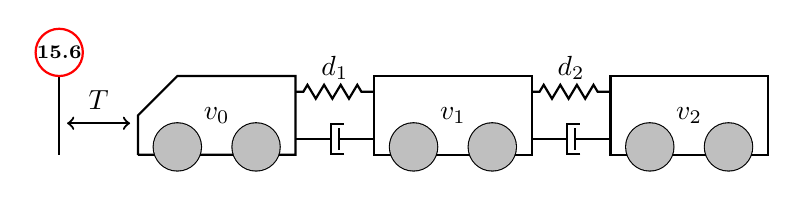
\begin{tikzpicture}
      \tikzstyle{spring}=[thick,decorate,decoration={zigzag,pre length=0.1cm,post length=0.1cm,segment length=6}]
\tikzstyle{damper}=[thick,decoration={markings,
  mark connection node=dmp,
  mark=at position 0.5 with
  {
    \node (dmp) [thick,inner sep=0pt,transform shape,rotate=-90,minimum width=10pt,minimum height=2pt,draw=none] {};
    \draw [thick] ($(dmp.north east)+(2pt,0)$) -- (dmp.south east) -- (dmp.south west) -- ($(dmp.north west)+(2pt,0)$);
    \draw [thick] ($(dmp.north)+(0,-4pt)$) -- ($(dmp.north)+(0,4pt)$);
  }
}, decorate]
\draw[thick] (0, 0) -- (2, 0) -- (2, 1) -- (0.5, 1) -- (0, 0.5) -- (0, 0);
\draw [spring] (2, 0.8) -- (3, 0.8);
\draw [damper] (2, 0.2) -- (3, 0.2);
\draw[thick] (3, 0) rectangle (5, 1);
\draw [spring] (5, 0.8) -- (6, 0.8);
\draw [damper] (5, 0.2) -- (6, 0.2);
\draw[thick] (6, 0) rectangle (8, 1);
\draw[thick] (0.5, 0.1) circle (0.3);
\fill[color=lightgray] (0.5, 0.1) circle (0.3);
\draw[thick] (1.5, 0.1) circle (0.3);
\fill[color=lightgray] (1.5, 0.1) circle (0.3);
\draw[thick] (3.5, 0.1) circle (0.3);
\fill[color=lightgray] (3.5, 0.1) circle (0.3);
\draw[thick] (4.5, 0.1) circle (0.3);
\fill[color=lightgray] (4.5, 0.1) circle (0.3);
\draw[thick] (6.5, 0.1) circle (0.3);
\fill[color=lightgray] (6.5, 0.1) circle (0.3);
\draw[thick] (7.5, 0.1) circle (0.3);
\fill[color=lightgray] (7.5, 0.1) circle (0.3);
\node at (1, 0.5) {$v_0$};
\node at (4, 0.5) {$v_1$};
\node at (7, 0.5) {$v_2$};
\node at (2.5, 1.1) {$d_1$};
\node at (5.5, 1.1) {$d_2$};

      \draw[thick] (-1, 0) to (-1, 1);
      \draw[thick,color=red] (-1, 1.3) circle (0.3);
      \node at (-1, 1.3) {\scriptsize \bf 15.6};
      \draw[thick, <->] (-0.9, 0.4) to (-0.1, 0.4);
      \node at (-0.5, 0.7) {$T$};
    \end{tikzpicture}
  \end{center}
\end{frame}

\begin{frame}{Results}
  \begin{columns}
    \begin{column}{0.55\textwidth}
      \begin{center}
        \includegraphics[width=\textwidth]{CruiseControlSets.pdf}
        \includegraphics[width=\textwidth]{CruiseControlBenchmark.png}
      \end{center}
    \end{column}
    \begin{column}{0.55\textwidth}
      \begin{center}
        \includegraphics[width=\textwidth]{CruiseControlSpeed.pdf}
        \includegraphics[width=\textwidth]{CruiseControlAcceleration.pdf}
      \end{center}
    \end{column}
  \end{columns}
\end{frame}

\section{Conclusion}

\begin{frame}{Conclusion}
  \begin{block}{Conclusion}
    \begin{itemize}
      \item Safe MPC either needs long horizon or precomputed controlled invariant sets;
      \item Polyhedral computation of controlled invariant sets is computationally intensive;
      \item Ellipsoidal computation of controlled invariant sets is semidefinite representable in the dual space.
    \end{itemize}
  \end{block}
  \begin{block}{Future work}
    \begin{itemize}
      \item \alert{Semialgebraic} invariant sets using \alert{Sum-of-Squares}.
      \item Improve \alert{BMI} optimization for \alert{non-symmetric} case.
      \item \alert{Piecewise} quadratic invariant set.
    \end{itemize}
  \end{block}

\end{frame}

\end{document}
